\chapter{Civic Mobile Learning: Theory and Practice}
\label{chap:MobileLearning}

This chapter gives an overview of the previous research that has been conducted concerning mobile learning and influenced the design of the technology created for this project. The learning theories of constructionism and project-based learning are also covered, as they are particularly important to the research discussed in \autoref{chap:student-created}.

\section{Civic Learning in Space and Place} 

The importance of space and the context of place in educational processes is a well-researched subject. Dewey recognised the educational potential and underuse of physical and social environments outside of the classroom in 1938, noting that the physical, historical, occupational and economic conditions of the local community could be utilized as learning resources \citep{Dewey1938}. Prior research has highlighted the advantages of authentic learning contexts, particularly in relation to place-making and preparing learners for active citizenship.

\subsection{Situated Outdoor Learning}
Lave and Wenger's Situated Learning Theory posits that learning is normally situated: embedded within activities, contexts and cultures \citep{lave1991situated}. They argue that social interaction and collaboration become essential for the learner to assume a role of expertise, by moving from the periphery to the centre of `communities of practice' (a group of people either virtual or in-person, who share a craft, profession or common interest) through `legitimate peripheral participation'. This participation for newcomers could initially consist of simple, low-risk tasks which further the goals of the community. As the newcomers gain experience and are recognised for their mastery of tasks, they move towards to the centre of the community and become `old-timers' to new members. Lave and Wenger argue that collaboration and social interaction are essential components of learning, which lead to learners entering a relevant community of practice. This ideal is in clear contrast to more traditional classroom activities, where knowledge commonly isn't presented in authentic contexts. Lave argues: `\textit{Once one begins to think in terms of legitimate peripheral participation in communities of practice, many other forms of socially organized activity become salient as sites of learning. But if one turns to formal, explicit, salient educational sites, it is difficult to identify communities of practice, widespread mastery, and traditions of centripetal participation leading to changing identities of mastery}' \citep{Lave1991}. As such, Situated Learning Theory places emphasis on legitimate peripheral participation in communities of practice, focusing on the relationship between learning and the social situation in which it occurs \citep{lave1991situated}. It follows that meaningfully engaging within these communities can also be framed as a place-making process: it exposes learners to others' interpretations of place, as well as encouraging them to develop their own interpretations through the growth of new relationships with existing communities. Furthermore, it means that for a large number of subjects and communities the classroom is not an ideal learning environment.

As shown in the previous chapter through the discussion of projects such as Remix Portal, communities can be a significant source of knowledge and expertise, often underused by formal education systems \citep{Dodds2017}. However, there exists a danger of simply framing local experts as taking a fairly passive role with regards to knowledge sharing---a knowledge resource to be sapped, rather than stakeholders with their own motivations and agendas. Communities can also actively create new learning material: to encourage the capitalisation of local knowledge, Leat argues for the introduction of community curriculum making \citep{Leat2015}. This involves a portion of a school's curriculum being developed alongside community partners and making use of community resources. Leat claims that not only do students find working alongside community members to be more compelling and engaging, but that exposure to these new individuals can also provide new opportunities for identity development. As with the contrast between the ideals of situated learning and the classroom-based reality, Leat notes that the current curriculum-focused schooling system is configured in a way that creates strong pressures to `teach to the test'. He argues that this has created a gulf between in-school and out-of-school learning, with schools introverting and over-emphasizing the value of `official' curricula, pedagogy and assessments. As a result, schools aren't fully engaging with local resources, opportunities, issues and needs---removing opportunities for students to discover and enter nearby communities of practice.

However, engaging with physical local resources found in space as educational resources has gained popularity within the last few years. Outdoor learning (also commonly referred to as ‘learning outside the classroom’ \citep{Lotc.org2006}) is an experiential approach to learning which develops personal, social and environmental understanding and skills, with outdoor environments being core to the experience \citep{Harvey2012}. While for some subjects outdoor learning activities don't class as situated learning (for example, the scheme  `Computer Science Unplugged' can take place outdoors in a playground, instead of the `authentic context' of a computer development environment \citep{Bell2009}), the two are clearly intrinsically linked when the subject matter concerns outdoor resources which are accessible to the learner. The benefits of outdoor learning have been extensively researched and recognised. In their 2015 review of the evidence base surrounding outdoor learning, Fiennes et al. found that nearly all of the papers they reviewed reported that outdoor learning activities had consistently positive effects: on everything from children's academic performance to social skills and self-image \citep{Fiennes2015}. In their 2008 report, the UK government's Office for Standards in Education, Children's Services and Skills (Ofsted) noted that `\textit{Learning outside of the classroom contributed significantly to raising standards and improving pupils’ personal, social and emotional development}', finding that `\textit{Hands-on activities led to improved outcomes for students, including better achievement, standards, motivation, personal development, behaviour [and] positive effects on young people who were hard to motivate}' \citep{Ofsted2008}. As a result, they labelled outdoor learning as an essential element of a broad and balanced curriculum and are urging schools to make explicit reference to it in their self-evaluation.

\subsection{Civic Learning}
Civic learning is an essential component in educational systems wishing to promote active citizenship within society. For the purposes of this research, civic learning is defined as being that which supplies the learner with the knowledge, skills and values they need to be citizens who actively participate in their local communities and take responsibility for improving and understanding them. However, despite `Citizenship Education’ (a subject within the UK’s education system dedicated to civic learning) being shown to have positive influences on political efficacy, participation, involvement and knowledge \citep{whiteley2012}, it has been demoted within the UK’s Department of Education to an optional subject as a part of the Basic Curriculum \citep{GovEducation2011}. It is now recommended to be included within other curriculum areas rather than as a distinct `subject’, despite previous findings showing it had already suffered from delivery by non-specialist teachers and being treated as a second-tier subject due to its lack of formal assessments \citep{Burton2015, Ofsted2013}. Burton even speculates that this neutering of civic learning in the UK may be a deliberate action by policy makers to avoid encouraging democratic debate, freethinking and ‘\textit{engendering extensive controversy and potential anti-establishment action}’ \citep{Burton2015}. It's not unlikely that a lack of quality civic education would impact the students' future roles as active citizens. This further highlights the educational importance of Digital Civics (and the adjacent concepts, such as spatial citizenship education) and how digital technologies can play a role in preparing students for their futures roles as citizens.

\section{Mobile Learning}
Mobile learning (m-learning)—which Crompton et al. define as `\textit{learning across multiple contexts, through social and content interactions using personal electronic devices}'\citep{Crompton2013}—has been increasingly of interest in HCI due to the growing abundance of mobile devices. The portability and networking capabilities of these devices has been shown to be of great potential for educational applications: not only allowing users to access online learning materials irrespective of time and place, but also allowing m-learning applications to take advantage of the user’s physical environment to enhance the learning experience \citep{Frohberg2009}. The adoption of mobile devices into UK classrooms has been dramatic, with nearly half of UK schools being expected to have one tablet per child within the next few years \citep{BritishEducationalSuppliersAssociation2015}. While traditional desktop and laptop devices are currently still more common in schools \citep{BritishEducationalSuppliersAssociation2017}, mobile devices have been touted as having a number of advantages over their more stationary counterparts: for example, Traxler argues that mobile technologies can offer structured educational experiences which can be situated in---and responsive to---authentic learning environments \citep{Traxler2011}. This makes mobile learning well suited for situated learning practices. Previous m-learning research has used these capabilities for a wide variety of applications, such as sensing tool kits to conduct citizen science \citep{Sharples2017}; enabling seamless learning across classrooms and museums on school trips \citep{Vavoula2009}; and empowering children in collecting evidence to support their advocacy and engagement in urban design processes \citep{Peacock2018}. This section will explore some previously undertaken work, including explorations of the potential pedagogical roles of m-learning technologies and how existing projects have put these theories into practice.

\subsection{Activity Theory and the Task Model for Mobile Learning}
A variety of social and environmental resources and influences must be considered when designing mobile learning activities, due to the portable nature of the devices they inhabit. Activity Theory has long been used as a framework through which the impacts and interactions of a variety of factors affect an activity’s process and results (Figure \ref{fig:taskModelMLearning}). The second generation of the framework describes a system for performing an activity---where a subject (e.g. a student) works on an `object' (e.g. a book report) in order to obtain a desired outcome (e.g. a completed review of a book for class), using tools and `instruments' which can be internal (e.g. prior knowledge) or external (e.g. online resources) \citep{leont1978}. In order to consider multiple people working on the same object, Engestr{\"o}m extended the framework by adding a `community' component, featuring `rules' (explicit and implicit definitions of how subjects should fit into the community) and `division of labour' (how the activity's object relates to the community) \citep{Engestrom2001}. Engestr{\"o}m's third generation of Activity Theory represents the multiple perspectives of community members through the binding of multiple of these activity systems over a common object. As a result, this version of Activity Theory has become a valuable tool for analysing the processes of activities undertaken by individuals and groups.

\begin{figure}
\centering
  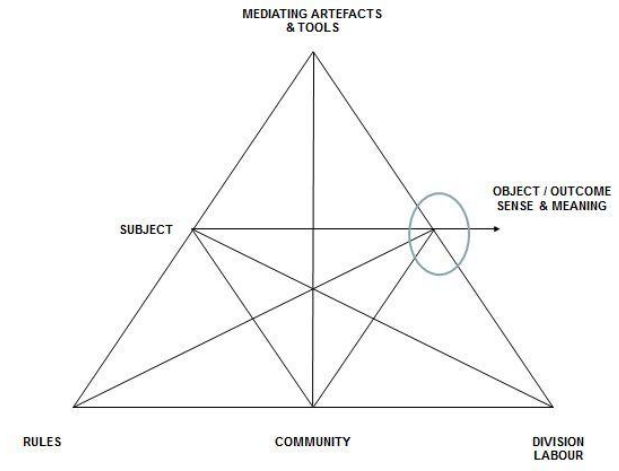
\includegraphics[width=0.8\columnwidth]{images/chapter03/activityTheory.PNG}
  \caption{The second generation of Activity Theory \citep{leont1978, Engestrom1987}. The third generation combines multiple of these triangle models through a potentially shared object \citep{Engestrom2001} }~\label{fig:activityTheory}
\end{figure}


However, this version of the framework still lacked the means to describe some of the factors involved when performing educational activities in space and place. With the aim of constructing a framework suitable for mobile learning, Sharples and Taylor extended the third generation of the framework further, creating a task model for mobile learning (TMML) which placed new emphasis on previously overlooked factors: context, control and communication \citep{Sharples2007,Taylor2006} (Figure \ref{fig:taskModelMLearning}). In this model, `context' refers to the learning environment (an important factor, considering the portability of mobile learning systems), `control' refers to the amount of scaffolding and moderation placed upon the learning activity, and `communication' describes the user’s interaction with other learners. Activity Theory’s subject, object and tool are still present, describing the learner, the learning object and what they will use to assist in that learning respectively. As this model allows for the description of any mobile learning project in a structured way, comparisons with other mobile learning projects are possible.

\begin{figure}
\centering
  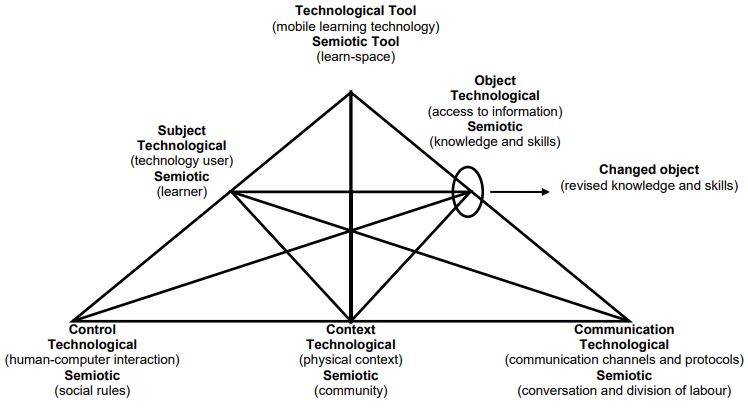
\includegraphics[width=1\columnwidth]{images/chapter03/taskModelForMobileLearning.PNG}
  \caption{A framework for analysing mobile learning \citep{Taylor2006}. Expanding upon Activity Theory, it adds Control, Context and Communication as additional factors to consider when designing for mobile learning.}~\label{fig:taskModelMLearning}
\end{figure}

Using the TMML, Frohberg et al. performed a critical analysis of mobile learning projects existing prior to 2008 which, while technologically outdated, still provides numerous insights applicable insights for design \citep{Frohberg2009}. The authors produced their review of existing projects by analysing them according to each of the TMML's factors: context, tools, control, communication, subject and object. Below is a brief overview of the discussions held by Frohberg et al. on each of the factors, as well as insights from other research.

\subsubsection{Context}
Frohberg uses \textit{Context} to describe the relationship between the learning context and the learner, placing activities into four categories: independent (when the learner's physical/social environment has no relationship to what they are learning), formalized (a formal education, classroom-like setting), physical (the learning takes place in a space relevant to the learning topic---the learning is physically authentically situated) and social (subjects learn through sharing sustainable relationships with others---e.g. entering a community of practice). 

Many of the projects examined by Frohberg et al. were found to exist independent of the learner’s context. A modern example could be the educational website Khan Academy, which aims to ‘\textit{provide a free, world-class education for anyone, anywhere}’ \citep{Khan2011}. As Khan Academy is location independent, it can’t take advantage of the learner’s current surroundings as an educational resource. Conversely, the Ambient Wood project used the physical context to provide learners with contextually-relevant digital information during their exploration of the environment, provoking reflection and discussion \citep{Rogers2004}. By categorising mobile learning projects by their contexts, Frohberg et al. also noted that most either took place independently of the learner’s environment or relied upon its physical properties alone. Few engaged in a `socializing' context, in which learners share relationships, emotions, values or personal history. Other examples can be found in mobile learning literature---for instance, while MOBIlearn attempted to incorporate the learner’s spatial and temporal contexts within a museum, it didn't engage with the social context: the museum’s role in the surrounding communities and the relationships it shared with their members \citep{Lonsdale2004}. Another example could be the Talking Statues project, which provides a passive civic learning experience by exposing the learner to underlying meaning and local knowledge through augmented reality: nearby celebrity-voiced statues ‘phone’ the learner to inform them about local histories \citep{Sing2017}. However, this passive interaction doesn't allow for much relationship building---one way to further embrace the social context of the statues could be to have learners contribute their own interpretations and stories relating to place. Such technologies could be suitable for the sharing of place meaning and empathetic place-making.

\subsubsection{Tools}
\textit{Tools} is the term used in the TMML to designate any material, medium, device, instrument or artefact that is used to mediate the learning process. For their critical analysis, Frohberg et al. produced a scale describing the learners' tool usage---from a passive, content consumption mode of learning on one end, to content construction on the other. They argue that while more passive learning tool usage is often more efficient for teachers (as content can be pre-prepared for delivery and can be easily assessed), it offers a cognitively passive learning experience through which the learner is unlikely to gain much more than a low-level of understanding and applied knowledge. In between these extremes lie simple interactions for motivation (such as quizzes), guided reflection through situated tasks to reflect upon, and reflective data collection, in which learners explore an environment to collect their own data. 

Frohberg et al. found that many the analysed projects provided extremely passive learning experiences, delivering content to the user which offered little to no creative control over their learning or output. The authors noted that projects which leaned towards the learner constructing content (rather than passively experiencing existing content, such as video, written articles, podcasts or---to a lesser extent---multiple-choice quizzes) offered the learner a deeper understanding through reflection. Chan et al. argue that the delivery of simple `instructional content' results in the learner being regarded as simply a consumer of product, ignoring the high pedagogical value of active, productive, creative and collaborative learning \citep{Chan2006}. Examples of activities that have tools which promote reflection through creativity include solving the open questions found within digital mysteries \citep{Kharrufa2010}, and children’s creation of digital ‘hidden stories’ to be shared with others \citep{Wood2014}. Passive delivery of content is unlikely to provoke deep learning and civic engagement: as with Gryl and Jekel’s technologies for spatial citizens, effective civic technologies should allow learners to actively engage in dialogues surrounding places’ meanings and social infrastructures, rather than act as a simple information delivery system \citep{Gryl2012}.

\subsubsection{Control}
The TMML adds \textit{Control}, which describes the balance of responsibility between the teacher and the learners for the learning process and setting targets. As with Tools, Frohberg et al. placed the projects they analysed on a spectrum, from tight teacher control to full learner control. They note that while full teacher control is efficient for delivering specific content, it offers learners very little responsibility, impacting motivation and introducing the danger of learners `doing the motions' without deep understanding of the content. However, they argue that the opposite end of the scale also risks over-straining learners, with a lack of oversight potentially leading to disorientation, missed learning goals, frustration or the development of false conclusions. As a result, Frohberg argue that somewhere between the two would be preferable, with a degree of scaffolding or direction still being required in most cases. Land similarly stresses the necessity of scaffolding and offers multiple other mobile learning design guidelines, including supporting a range of learner ages and reading abilities through visually varied interfaces \citep{Land2015}. Frohberg found that few of the mobile learning projects they analysed were positioned in this ideal scaffolding range, with most having overbearing teacher control and a few having less learner-orientation than would be ideal. They note: `\textit{very few Mobile Learning projects with physical context explicitly considered, positioned or focused the usage of mobile technology as instruments to gain transparency and steer flexible learning activities there}', arguing that achieving the full potential for m-learning technologies may require allowing learners more space and freedom, whilst still offering a degree of guidance.

\subsubsection{Communication}
Representing the `community' element of Activity Theory, \textit{Communication} in TMML refers to if and how the learner works with others during the learning process. Frohberg et al. argue that reflection can be encouraged by learners working together, identifying and filling each other's knowledge gaps to achieve deeper learning. The authors again place the degrees of communication found in each project on a scale. The extreme low end of this scale features isolated learners who work independently with the learning material and given tools. Following this are `loose pairs' of students, who work on the same device or learning material, but the learning scenario doesn't explicitly require them to cooperate---students asked to work together and discuss a piece of work are `tight pairs'. The upper tiers of the scale denote pairs working within larger teams, and then communication and cooperation between teams to work on common object. Frohberg et al. argue that most of the projects they reviewed focused on learning scenarios with low communication and interaction, and that these projects missed out on potential for deeper learning and reflection.

\subsubsection{Subject \& Object}
Frohberg et al. argue that a vast majority of the mobile learning projects they analysed were engaging with novices with little-to-no prior knowledge as the subject (learner). The authors suggest that while novice learners are often easier for researchers to acquire and work with, novices are not usually expected to be able to perform higher forms of learning such as applying knowledge and reflection. As a result, they note a lack of research regarding systems where the object targets more experienced subjects.


\subsection{Engaging Infrastructures of Place with Mobile Learning}
While many m-learning projects have excelled at teaching many ‘traditional’ curriculum subjects which often focus on physical environmental properties (such as biology, history and geography), few existing m-learning technologies capitalise on the embedded social value of their settings, thus potentially missing out on a wealth of civic learning resources. Additionally, while some previous research has explored how technologies can enhance and develop meaningful relationships with space and place \citep{Giaccardi2008, Lentini2010} or support existing classroom activities \citep{Mann2016}, little work has explored how technologies and design processes can utilise relational infrastructure for civic m-learning in public places. As noted by Frohberg et al, it appears that few mobile learning research projects have considered and exploited the multiple layers that comprise space and place: looking beyond their physical properties and engaging the learner with the socio-cultural, economic and political practices within civic space \citep{Frohberg2009}. It stands to reason that technologies designed for civic learning would likely benefit from the application of situated learning in authentic social and physical contexts. Leat's `community curriculum' could be one possible way to achieve this: a place’s stakeholders can also be valuable resources for civic mobile learning, acting as potential routes to introducing learners to new communities of practice and establishing community curricula \citep{Leat2015}.

Balestrini et al's CrowdMemo project engaged with the socio-cultural infrastructures of civic space in an educational context, using mobile technology as a platform for community storytelling \citep{Balestrini2014}. This study was particularly notable due to the community's strong uptake of project, and the levels of engagement displayed by stakeholders. The authors report that a key factor in the participants' engagement with the project was that they felt recognised and valued, both from inside and outside of their local community. One of the teachers noted that \textit{`[the elderly people] who were interviewed by the students expressed enthusiasm and excitement, because they were being recognised for what they had done.'} The authors argue that the other main contributing factor was that the project provided value to all of the project's stakeholders. This includes the school students, the teachers, the elders and even the researchers. Each of these groups had their own needs and agendas, which needed to be fulfilled in some way in order to encourage meaningful participation and engagement. For example, some members of the community had a growing concern that failure to document and preserve the town's architectural heritage could threaten its future legacy and its identity going forward. Teachers were keen to provide new innovative and effective teaching techniques and content. Students valued being able to use technology for schoolwork which had normally been considered `contraband', and learning new ways of utilising their devices. It appears that many of the elders simply wanted to be valued, and enjoyed being able to share their past experiences with younger generations who could keep their memories alive. Each of these motivations will have shaped those stakeholders' approaches and attitudes towards their involvement with the project. There is also a hint within the authors' report that the intersections of these motivations and experiences can provide excellent learning opportunities: for example, they note that \textit{`the children were very keen to teach adults how to access the documentaries by scanning codes'}. In this instance, it wasn't only the elders passing knowledge down, but the children sharing their own with them in exchange.

HCI research has also explored how stakeholders can highlight their knowledge, values and identity through the creation of digital technologies outside of the context of mobile learning. For example, Fox and Le Dantec's `Community Historians' project explored how communities' power dynamics could be examined through the participatory design of technology with disenfranchised communities `\textit{not typically empowered to voice their opinions, let alone create their own systems or devices}' \citep{Fox2014}. Through a series of workshops, the researchers explored how stakeholders can use the creation of technology to empower themselves and articulate community identity. They also argued that creating opportunities for non-experts to directly manipulate specialised materials (in this case, computer components and sensors) would allow stakeholders to gain a crash-course in understanding how those technologies work and could be used within their community. They argued that this `democratisation' of technology creation created new opportunities for community stakeholders to create technologies according to their own needs and values: 
\textit{`The potential of [accessible prototyping systems], and the aspirations of those who create them, turn on the ability to shift the dynamic away from the consumption of corporate-designed devices towards a more egalitarian structure of user-as-designer.'}

\subsection{Seamless Mobile Learning}
\label{sec:Seamless}

\begin{figure}
\centering
  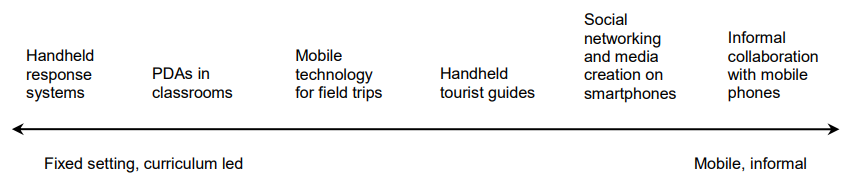
\includegraphics[width=1\columnwidth]{images/chapter03/learningContextDimension.PNG}
  \caption{ Sharples' example of types of mobile learning, plotted on a linear dimension from a formal and fixed learning context, to one that is mobile and informal \citep{Sharples2013}. }~\label{fig:learningContextDimension}
\end{figure}

Sharples presents mobile learning as existing on a linear dimension from a fixed, curriculum-led context on one end, to one of informal learning in a mobile setting on the other \citep{Sharples2013} (Figure \ref{fig:learningContextDimension}). Whereas a formal learning setting might be in an environment such as a classroom, informal learning is less limited, and frequently in a mobile context. He notes that connecting these formal and informal learning contexts provides new research opportunities for mobile learning, working towards Kuh’s proposed binding of different learning experiences into a single ‘seamless learning’ narrative, where the learning experiences are able to continue across multiple environments (and bridging formal/informal contexts) seamlessly \citep{Kuh1996}. Wong and Looi claim that seamless learning technologies ‘empower and support’ users in learning, whenever and wherever they are stimulated to do so \citep{Wong2011}. They identified ten desirable dimensions which characterise ‘seamlessness’ within mobile learning design: 1) encompassing formal and informal learning, 2) encompassing personalized and social learning, 3) learning across time and 4) locations, 5) ubiquitous access to knowledge, 6) encompassing physical and digital worlds, 7) using multiple types of devices, 8) switching between multiple learning tasks, 9) knowledge synthesis (e.g. combining learners’ prior knowledge with new knowledge) and 10) encompassing multiple pedagogical or learning activity models. They note that more research could be done to investigate how mobile learning technologies could support four of these qualities (7 - 10) and use them to facilitate holistic seamless learning experiences. 

\subsubsection{Seamless Mobile Learning in Practice}
In this section, we will briefly review how some other mobile learning projects, particularly focusing on projects which have supported seamless learning and the creation of user-generated content. In their investigation into the potential usage of mobile learning in rural Panama, Valderrama et al. found that ‘multimedia rich’ phones were welcomed by pupils and teachers for use in classroom activities, even without the installation of additional software applications \citep{ValderramaBahamondez2011}. However, as mobile app stores have gotten more popular, most other studies have focused on custom, education-focused mobile software installed on otherwise off-the-shelf devices. These apps frequently either consist of `toolkit' (where the device and software are used for data collection or analysis, and contain little-to-no teaching material) or more guided approaches (where learners are scaffolded through more specific learning material). 

The Sense-it mobile application takes takes the toolkit approach, foregoing any scaffolded structure and acting as free-form supporting tool \citep{Sharples2017}. It allows users to conduct citizen science (research conducted by amateur scientists, usually through public participation of data collection) investigations through accessing detailed sensor information from their phone’s hardware, without having any overarching activity scaffolding within the application itself. While alone it acts as an unstructured toolkit, Sense-it can be combined with the nQuire-it web platform to support users in contributing to others’ created investigations or even designing and completing their own. However, the nature of Sense-it’s citizen science focus means that the user interactions are limited to data collection activities, resulting in the mobile technology offering little creativity unless integrated into a larger project.

Mobilogue supports the authoring of location-based mobile learning activities, which linearly guide learners between locations using GPS and ask quiz questions at each one \citep{Giemza2013}. As with nQuire-it, Mobilogue’s website component allowed students greater control through creating their own quizzes for their peers. The authors noted that this provoked a `learning by teaching effect’, and that the students were particularly engaged by seeing their created quizzes in action on mobile devices. This supports Heslop et al., who argue that higher level thinking and reflection can be promoted in students through them creating ‘Digital Mysteries’ for each other \citep{Heslop2017}. Once finished, Mobilogue users can clear their progress, allowing devices to be shared amongst multiple students in a class. However, as learners’ responses in Mobilogue aren't uploaded for later review on other devices, opportunities for seamless learning through follow-up activities in other contexts are limited. This creative element was also only available on the website, with the mobile application’s delivery of passive content offering learners little control when examined using the mobile learning task model \citep{Taylor2006}.

Wild Knowledge expands on the toolkit and authoring concepts, supporting varied learner activities made up of modular components \citep{WildKnowledge2015}. These include photography, audio recording, location logging and interactions often found on standard worksheets such as multiple-choice questions. Through the platform’s website, users can combine these interactions into activities for others to complete. Learners can also upload their responses for later viewing on the website, where it is displayed in a comma separated (CSV) table format. This format would likely be too complicated for younger children, suggesting that Wild Knowledge was not designed as a seamless learning tool with this age group in mind. Other than being referenced in literature (e.g. \citep{Traxler2013}), I am not aware of any research that investigates the use of Wild Knowledge in educational contexts. Furthermore, the platform’s subscription model appears to focus on schools and businesses with a top-down delivery of content, rather than supporting individuals and communities in sharing information with a low financial barrier to entry (and engaging with social contexts for civic learning).

An example of a mobile learning technology designed for seamless learning is the MyArtSpace project, which created a seamless learning experience between a school trip to a museum and follow-up classroom activities, through the combination of a website and mobile application \citep{Vavoula2009}. Using the application, students `collected’ digital content linked to physical items in the museum in response to an inquiry question. Learners could also upload their own images, text and audio recordings during the visit. On return to the classroom, students could review their collected content and use it to answer their given question. The technology successfully bridged the museum and classroom learning contexts, and increased levels of student engagement and reflection upon return to the classroom. 

Following in the footsteps of MyArtSpace is Zydeco, another platform designed to support seamless mobile learning \citep{cahill2010, kuhn2011}. Zydeco is a learning platform---comprising of a mobile application and a website---designed to help link classrooms with museum contexts, by supporting greater integration of activities between the two. The authors argue that the authentic learning materials and interactive exhibits frequently present in museums make them ideal contexts for student-driven inquiry, but that this can frequently clash with the structured teaching style found in formal classroom learning. Zydeco aims to assist with this by supporting structured (but not overly limited) activities during museum trips, which the authors argue supports students in making `\textit{cognitively-fruitful inquiry}' and conceptual connections to previous classroom activities. By using the website in the classroom environment, students and teachers are able to define goals and questions related to particular scientific investigations. This information is then able to be transferred to the mobile app, allowing students to respond to the created prompts in situ on school trips by taking, tagging and annotating photos. While paper-based worksheets requiring excessive writing can interfere with students' experiencing the museum, the authors argue that interactions such as taking photographs and writing short tags are less intrusive and would detract less from the learning experience. After the trip has completed, the students can then access these responses in the classroom to seamlessly continue their investigations. Through seamless learning, the authors argue that the application was able to utilize the affordances of both the classroom (structured, guided, formal, teacher-led) and the museum (exploratory, inquiry-based, more informal and student-led), by mediating the latter through a layer of scaffolding to assist the learners going to and from the former.

However, these projects are somewhat limited in their scope for what the learner can use them for when in authentic learning environments. For example, MyArtSpace has only a limited ability for rich, reflective data capture: users can only create 15 second audio recordings, meaning that learners are limited to simply cataloguing information, rather than reflecting upon it in situ. In this way, the recordings functioned as an audio equivalent of the photo tags and descriptions possible in Zydeco, which are again too limited for rich reflection, for which additional engagement upon return to the classroom would be required. Additionally, the applications' exclusive focus on indoor environments such as museums and galleries limits the scope of their activities, as it precludes elements such as location-based interactions. The MyArtSpace project was also reported to suffer from usability issues resulting from the app’s reliance on typing and the website’s interface. These elements would likely be somewhat mirrored with Zydeco, as it also relies on students inputting text with mobile devices. As a result, there seems to still be an under-explored potential for seamless mobile learning platforms which allow the creation of semi-structured learning activities which promote reflection in authentic learning environments.


\section{Constructionism and Project-Based Learning}
\label{sec:ConstructionismPBL}

The learning theory of constructionism, introduced by Seymour Papert in the mid-1980s, argues that constructing, sharing and reflecting upon physical or virtual `public entities' (which could range from physical artefacts such as models of buildings, to virtual programming code or even conceptual theories of the universe) can be a powerful way for learners to build `knowledge structures'---collections of knowledge, concepts and facts interrelated through various semantic relationships \citep{PapertSeymourandHarel1991a}. Papert argues that the process of learning is the building of these knowledge structures, a process which--while it occurs irrespective of the circumstances of the learning--happens `\textit{especially felicitously in a context where the learner is consciously engaged in constructing a public entity}'. 

In their overview of constructionism, Noss and Hoyles argue that constructionist working environments offer a medium in which learners can `\textit{explore and learn from feedback, much as one can master a foreign language by living in the appropriate country}' \citep{Noss2017}. Noss and Hoyles also claim that they afford learners to take ownership of a construction-based approach, potentially leading to greater engagement, confidence and empowerment. Finally, they posit that through exploration and construction of public entities, learners can encounter `powerful ideas': `\textit{concepts and strategies  that confront and build upon intuitive knowledge}'. For this reason, Noss and Hoyles argue that constructionist tools need to be expressive enough to facilitate these ideas emerging through the learner's construction of public entities.

Project-based learning (PBL) is an instructional pedagogy which presents learners with a given `problem' or task, requiring them to investigate and work on a given subject over a longer period of time. These problems are non-trivial and often framed as `authentic', in that they are somewhat applicable to the real world \citep{Blumenfeld1991}. Frequently, students' projects will result in the creation of an artifact in response to the given problem (such as videos, reports, artworks, websites or performances \citep{Holubova2008}), in effect making PBL a method of applying constructionism in response to real-world problems and supporting the inclusion of prior knowledge, domain research and greater levels of student autonomy. It's worth noting that several other configurations of pedagogy adjacent to PBL have been developed over time (e.g. problem-based learning), however they mostly conform to the same essential elements: a challenging problem or question; sustained inquiry; an element of authenticity; a degree of student control; reflection; critique and revision; and a final public product \citep{Larmer2015}. Previous research has argued that these projects can serve to build bridges between classroom activities and real-life experiences \citep{Blumenfeld1991}, enhance applied and conceptual knowledge around a subject \citep{Boaler1999}, and that greater levels of autonomy and challenge can result in higher levels of student engagement \citep{Wurdinger2007}.

While some studies have found that project-based instruction is not necessarily more demanding in terms of teaching time and resources \citep{Al-Balushi2014}, Blumenfeld et al. posit that by their nature PBL requires student engagement over extended periods of time \citep{Blumenfeld1991}. Krajcik et al. argue that constructing knowledge in meaningful and situated activities can take students more time, leading to teachers being hesitant to put it into practice when faced with strict and competing curriculum goals \citep{Krajcik2006}. The non-profit organisation Innovation Unit note `\textit{[PBL] can be a powerful learning strategy if it is part of a whole school change process, and [schools] are ready and able to make the necessary time and staff available}' \citep{InnovationUnit2016}, suggesting that putting PBL into practice requires substantial changes in how teachers approach classroom structures, activities and tasks. This is easier said than done, as governmental pressures and restrictions frequently placed upon UK teachers often limit the amount of time they can dedicate to particular topics and experiential learning methodologies which don't target given examinations (particularly in later school years, which place greater emphasis on quantifiable assessment) \citep{Ofsted2018}.

\subsection{Mobile Learning and PBL}
Project-based learning is recognised as a fertile ground for technology-enhanced learning. Bell argues that as long as it doesn't become the learning focus, technology can benefit all aspects of PBL (including research and data collection, knowledge sharing and artefact creation), and that tapping into students' existing computer fluency can boost engagement \citep{Bell2010}. ChanLin describes how students used digital technologies within PBL for researching on the web, taking photographs, participating in online communities and creating web pages as final artefacts \citep{ChanLin2008}. Heslop et al. found that the creation and sharing of interactive digital artefacts supported metacognitive skills, such as writing for an audience \citep{Heslop2017}. Sarangapani et al. explored how students could create interactive digital content as public entities to be shared with peers in other cultures, and argued that creating and sharing artefacts encouraged students to more deeply engage with the content \citep{Sarangapani2018}. However, these studies are of limited use for putting project-based mobile learning into practice, as they are either lab-based \citep{Heslop2017} or do not use mobile technologies for the creation of interactive content \citep{Sarangapani2018, ChanLin2008}.

Chan et al. note that the use of mobile technologies in PBL has been under-researched, but in their study noted that students used mobile devices for multiple stages of the PBL process, including researching on the Internet, making notes, sharing materials and making use of educational applications to help understand abstract concepts \citep{Chan2015}. Computing Science courses have also been adapted to PBL models, with students creating mobile technologies as their final public entities \citep{Massey2006, Rahman2018}. Massey et al. argue that this pedagogical approach aims to reframe the students as developers and decision makers of mobile applications, rather than simply end-users \citep{Massey2006}. Sarangapani et al. held studies in which students used mobile devices to create video recordings for cross-cultural PBL, noting that the schools claimed the resulting videos were accessible and engaging learning resources \citep{Sarangapani2016}. Students have also used Zydeco to use their research to prepare materials for use on school trips \citep{}. These studies suggest that m-learning technologies can be configured to support the PBL process, or even be used to construct the project's final public entity. With this in mind, we wanted to explore how m-learning technologies could be effectively utilised within PBL processes in schools, particularly in the process of students producing interactive public entities for other students as learning resources.

\section{Summary}
This chapter gave an overview of some of the previous research that has been undertaken regarding mobile learning technologies, as well as some of the theories which have influenced them.
An important factor which benefits mobile learning technologies is that they can be situated (outdoors, if needs be) in authentic learning environments, both physical and social. Lave and Wenger's Situated Learning Theory highlights the importance of learner participation in activities, contexts and cultures which are `authentic' to the subject being learned \citep{lave1991situated}. There has been a push for in outdoor learning in schools as a result---while not always actually `Situated Learning', evidence highlights the benefits benefits of schools simply engaging more with outdoor resources \citep{Fiennes2015}.

Lave also places an emphasis upon learners entering `communities of practice', moving from the community's periphery to its centre as they gain expertise over time \citep{Lave1991}. Previous Digital Civics projects have engaged with communities as sources of expertise (e.g. \citep{Dodds2017, Rainey2019}). However, interactions with these communities can exist as more than a simple extraction of knowledge, as they are place stakeholders with their own motivations and agendas. Leat argues for the introduction of `community curricula', where schools develop learning materials alongside community partners to make better use of community resources, highlight stakeholder voices and provide new opportunities for students to enter communities of practice.

Sharples and Taylor's task model for mobile learning extends previous iterations of Activity Theory \citep{Engestrom2001}, additionally emphasizing the learning environment, the balance of learner control vs guiding scaffolding, and the communication between learners \citep{Sharples2007}. Frohberg used this framework to perform a review of early mobile learning literature \citep{Frohberg2009}. He found that many m-learning projects exist independently of the learner's physical and/or social context, meaning that they miss out on many potential learning resources. Many projects also only offered passive learning experiences, which offered little in the way of learner creativity. He also suggested that mobile learning activities need to strike a balance between being overly scaffolded and too open, with students needing some guidance whilst maintaining a degree of creative control over their work.

`Seamless' mobile learning technologies connect multiple learning contexts, such as formal classrooms and more authentic and engaging environments such as museums or the outdoors. Projects such as Zydeco provide opportunities for creating and transitioning data across these contexts, while also offering learners degrees of scaffolding in more informal learning environments \citep{kuhn2011}. However, while many of these projects encourage data collection and note-taking in these authentic learning environments, they don't seem to encourage or enable learner reflection in situ---this is done back in the classroom, upon review of collected data.

Finally, project-based learning (PBL) is an instructional pedagogy which engages learners by engaging them with a problem or task \citep{Blumenfeld1991}. Over an extended period of time, learners research the given topic, and construct a `public entity' in response to it (e.g. a web page, video, artwork or performance \citep{Holubova2008}). PBL has been shown to build bridges between the formal classroom context and real-life experiences, and is particularly engaging thanks to students being given greater levels of autonomy. While the use of mobile technologies specifically within PBL is somewhat under-researched, there are clear opportunities for the use of even existing m-learning projects throughout the PBL process: from research, sharing materials to the construction of public entities.